\documentclass[11pt, oneside]{article}   	% use "amsart" instead of "article" for AMSLaTeX format
\usepackage{geometry}                		% See geometry.pdf to learn the layout options. There are lots.
\geometry{letterpaper}                   		% ... or a4paper or a5paper or ... 
%\geometry{landscape}                		% Activate for for rotated page geometry
%\usepackage[parfill]{parskip}    		% Activate to begin paragraphs with an empty line rather than an indent
\usepackage{graphicx}				% Use pdf, png, jpg, or eps� with pdflatex; use eps in DVI mode
								% TeX will automatically convert eps --> pdf in pdflatex		
\usepackage{amssymb}
\usepackage{amsmath}
\usepackage{parskip}
\usepackage{color}
\usepackage{hyperref}

\title{Complex cosine and sine}
%\author{The Author}
%\section{}
%\subsection*{}
\date{}							% Activate to display a given date or no date

\graphicspath{{/Users/telliott_admin/Dropbox/Tex/png/}}
% \begin{center} 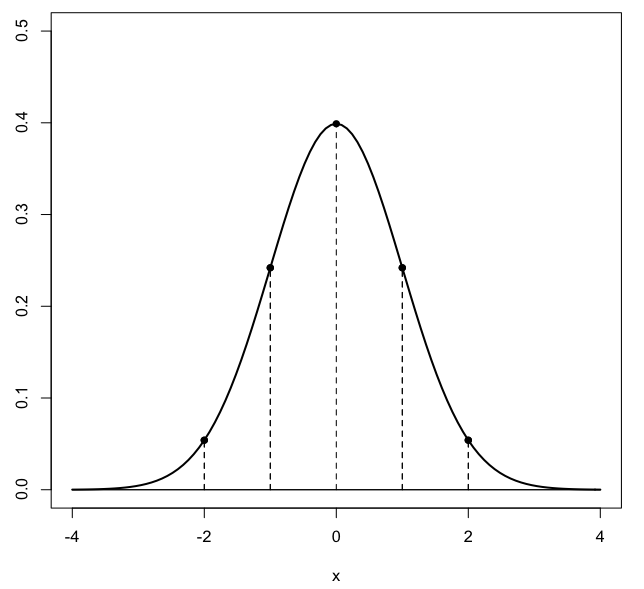
\includegraphics [scale=0.4] {gauss3.png} \end{center}
\begin{document}
\maketitle
\Large

We can define the complex counterparts of the real trigonometric functions similarly to their real equivalents by saying (again) that Euler's formula is also good for a complex number $z$.  So
\[ e^{iz} = \cos z + i \sin z \]
\[ e^{-iz} = \cos -z + i \sin -z = \cos z - i \sin z \]
This leads to:
\[ e^{iz} + e^{-iz} = 2 \cos z \]
and
\[ e^{iz} - e^{-iz} = 2i \sin z \]

On the other hand, Shankar defines them using series in the same way as the real versions:
\[ \sin z = \sum_0^{\infty} (-1)^n \frac{z^{2n+1}}{(2n +1)!} \]
\[ \cos z = \sum_0^{\infty} (-1)^n \frac{z^{2n}}{(2n)!} \]
\[ \sinh z = \sum_0^{\infty} \frac{z^{2n+1}}{(2n +1)!} \]
\[ \cosh z = \sum_0^{\infty} \frac{z^{2n}}{(2n)!} \]
and showing that they converge for any $z$.

A nice property for this definition of cosine is that
\[ \cos z = \frac{1}{2} \ (e^{iz} + e^{-iz}) \]
so
\[ \cos (z + 2\pi) = \frac{1}{2} \ (e^{iz}e^{i2\pi} + e^{-iz}e^{-2\pi}) \]
but
\[ e^{i 2 \pi} = \cos 2 \pi + i \sin 2 \pi = 1 = e^{-i 2 \pi} \]
so
\[ \cos (z + 2\pi) = \cos z \]
The \emph{period} of the complex cosine (and the complex sine) is $2 \pi$.

Take derivatives
\[ \cos z = \frac{1}{2} \ (e^{iz} + e^{-iz} ) \]
\[ \frac{d}{dz} \ \cos z = \frac{1}{2} \ (i e^{iz} - i e^{-iz} ) \]
\[ = \frac{i}{2} \ 2i \sin z = \sin z \]
Similarly
\[ \sin z = \frac{1}{2i} \ (e^{iz} - e^{-iz}) \]
\[ \frac{d}{dz} \ \sin z = \frac{1}{2i} i (e^{iz} + e^{-iz}) = \cos z \]
\subsection*{hyperbolic connection}
\[ \cos z = \frac{e^{iz} + e^{-iz}}{2} \]
if we consider $z = iy$ then
\[ \cos iy = \frac{e^{i^2y} + e^{-i^2y}}{2} \]
\[ = \frac{e^{-y} + e^{y}}{2} \]
But this is just $\cosh y$.  That is:
\[ \cos iy = \cosh y \]
Similarly
\[ 2i \sin iy = e^{i^2y} - e^{-i^2y} \]
\[ = e^{-y} - e^{y} \]
\[ = - (e^y - e^{-y}) \]
\[ = -2 \sinh y \]
Hence 
\[ i \sin i y = -\sinh y \]
\[ \sin i y =  i \sinh y \]
So what this means is that
\[ \cos z = \cos x + iy \]
\[ = \cos x \cos i y - \sin x \sin i y \]
\[ = \cos x \cosh y - i \sin x \sinh y \]
and what's nice about this is that we have the real and imaginary parts of the complex cosine easily visible.  Similarly
\[ \sin z = \sin x \cosh y + i \cos x \sinh y \]

\subsection*{analyticity}

We proved above that the complex exponential is analytic.  There is a theorem that says that if we add two analytic functions together, the result is also analytic.  Hence, the trigonometric functions are analytic.

But, just to check this result, let's write them out in terms of $u$ and $v$ and see whether the partial derivatives follow the CRE conditions:

\[ \sin z = \sin(x + iy) \]
By the addition formula
\[ = \sin x \cos iy + \sin iy \cos x \]
where $x$ and $y$ are real.

Recalling the result for the hyperbolic sine and cosine from above
\[ \cos iy = \cosh y \]
\[ \sin i y =  i \sinh y \]
then
\[ \sin z = \sin x \cos iy + \sin iy \cos x \]
\[ = \sin x \cosh y + i \cos x \sinh y \]
Taking the derivatives:
\[ u(x,y) =  \sin x \cosh y \]
\[ u_x = \cos x \cosh y \]
\[ u_y = \sin x \sinh y \]
and
\[ v(x,y) = \cos x \sinh y \]
\[ v_x = - \sin x \sinh y \]
\[ v_y = \cos x \cosh y \]
So we see that
\[ u_x = v_y \]
\[ u_y = -v_x \]

The CRE are satisfied and therefore, the complex sine is analytic.

Similarly we have that 
\[ \cos z = \cos (x + iy) \]
\[ = \cos x \cos iy - \sin x \sin iy \]
\[ = \cos x \cosh y - i \sin x \sinh y \]
So
\[ u(x,y) =  \cos x \cosh y \]
\[ u_x = - \sin x \cosh y \]
\[ u_y = \cos x \sinh y \]
and
\[ v(x,y) = -\sin x \sinh y \]
\[ v_x = -\cos x \sinh y \]
\[ v_y = -\sin x \cosh y \]
So we see that
\[ u_x = v_y \]
\[ u_y = v_x \]
Thus the complex cosine is also analytic.

We can also prove that:

\[ \sin^2 z + \cos^2 z = 1 \]
The easy way is
\[ \cos^2 z + \sin^2 z = \ [ \frac{e^{iz} + e^{-iz}}{2} \ ]^2 +  [ \frac{e^{iz} - e^{-iz}}{2i} \ ]^2 \ ] \]
\[= \frac{e^{2iz} + 2 + e^{-2iz} - e^{2iz} + 2 - e^{-2iz} }{4} \]
\[ = 1 \]

\end{document}  